\subsection{Dodicesimo sprint}

\begin{minipage}{\textwidth}
  Di seguito è riportata la distribuzione delle ore per ciascun membro del team, accumulate in totali per persona e per ruolo:
  \begin{table}[H]
    \begin{tabularx}{\textwidth}{|c|*{6}{>{\centering}X|}c|}
      \hline
      \multicolumn{8}{|c|}{\textbf{Consuntivo orario}} \\
      \hline
      \textbf{Membro del team} & \textbf{Re} & \textbf{Am} & \textbf{An} & \textbf{Pt} & \textbf{Pr} & \textbf{Ve} & \textbf{Totale per persona} \\
      \hline
      Riccardo Cavalli & 0 & 0 & 1 & 3 & 3 & 1 & 8 \\
      \hline
      Raul Pianon & 1 & 0 & 0 & 6 & 2 & 1 & 10 \\
      \hline
      Martina Dall'Amico & 1 & 1 & 0 & 4 & 3 & 2 & 11 \\
      \hline
      Marco Cristo & 1 & 1 & 0 & 3 & 3 & 1 & 9 \\
      \hline
      Sebastiano Lewental & 0 & 2 & 0 & 3 & 3 & 2 & 10 \\
      \hline
      Mattia Zecchinato & 2 & 0 & 2 & 2 & 2 & 2 & 10 \\
      \hline
      Tommaso Stocco & 0 & 0 & 2 & 4 & 4 & 2 & 12 \\
      \hline
      \textbf{Totale ore per ruolo} & 5 & 4 & 5 & 25 & 20 & 11 & \textbf{70} \\
      \hline
    \end{tabularx}
    \caption{Sprint 12 - Consuntivo orario}
  \end{table}
  \end{minipage}

  \begin{figure}[H]
    \centering
    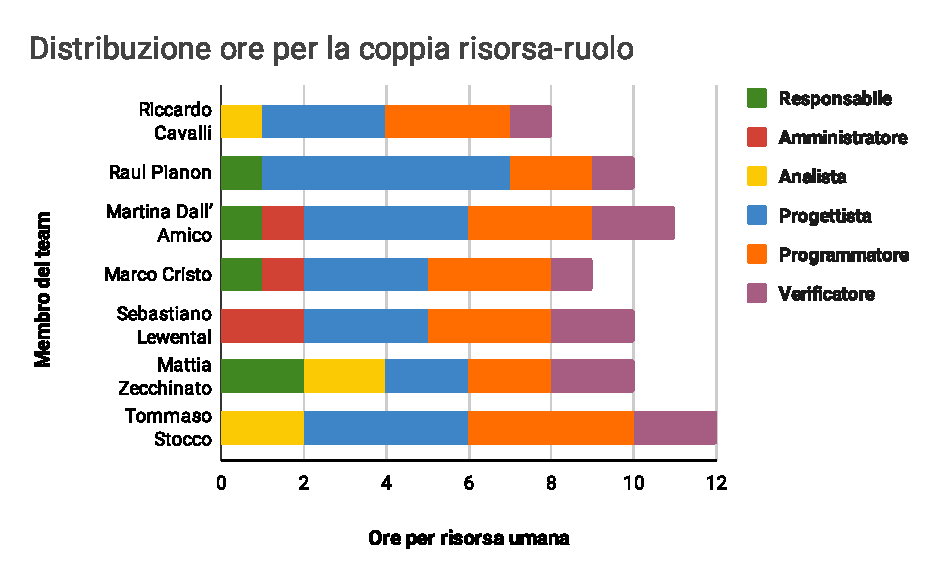
\includegraphics[width=0.90\textwidth]{assets/Consuntivo/Sprint-12/distribuzione_ore_risorsa_ruolo.pdf}
    \caption{Sprint 12 - Istogramma della distribuzione oraria per la coppia risorsa-ruolo}
  \end{figure}

  \begin{figure}[H]
    \centering
    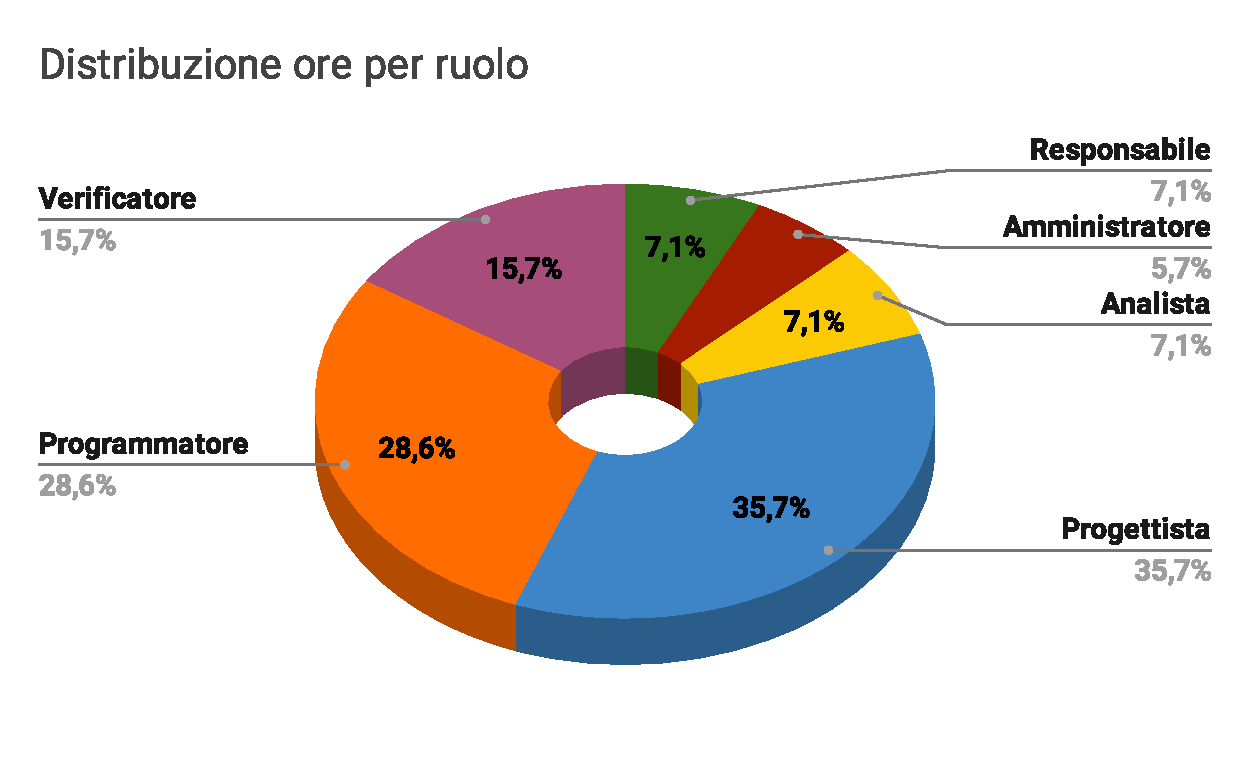
\includegraphics[width=0.90\textwidth]{assets/Consuntivo/Sprint-12/distribuzione_ore_ruolo.pdf}
    \caption{Sprint 12 - Areogramma della distribuzione oraria per ruolo}
  \end{figure}

  \begin{minipage}{\textwidth}
  Di seguito è riportato il consuntivo economico del dodicesimo \glossario{sprint}:
  \begin{table}[H]
  \begin{adjustwidth}{-0.5cm}{-0.5cm}
    \centering
    \begin{tabular}{|P{2.9cm}|P{2.3cm}|P{2.5cm}|P{2.3cm}|>{\arraybackslash}P{2.5cm}|}
      \hline
      \multicolumn{5}{|c|}{\textbf{Consuntivo economico}} \\
      \hline
      \textbf{Ruolo} & \textbf{Ore per ruolo} & \textbf{Delta ore preventivo - consuntivo} & \textbf{Costo (in \texteuro)} & \textbf{Delta costo preventivo - consuntivo (in \texteuro)} \\
      \hline
      \Responsabile[U]{} & 5 & 0 & 150,00 & 0,00 \\ \hline
      \Amministratore[U]{} & 4 & 0 & 80,00 & 0,00 \\ \hline
      \Analista[U]{} & 5 & 1 & 125,00 & 25,00 \\ \hline
      \Progettista[U]{} & 25 & -2 & 625,00 & -50,00 \\ \hline
      \Programmatore[U]{} & 20 & 1 & 300,00 & 15,00 \\ \hline
      \Verificatore[U]{} & 11 & 0 & 165,00 & 0,00 \\ \hline
      \textbf{Totale} & \textbf{70} & 0 & \textbf{1.445,00} & -10,00 \\ \hline
      \textbf{Restante} & 82 & / & 1.570,00 & / \\ \hline
      \textbf{Sprint pregressi} & 494 & / & 10.005,00 & / \\ \hline
    \end{tabular}
    \caption{Sprint 12 - Consuntivo economico}
  \end{adjustwidth}
  \end{table}
  \end{minipage}

  \begin{figure}[H]
    \centering
    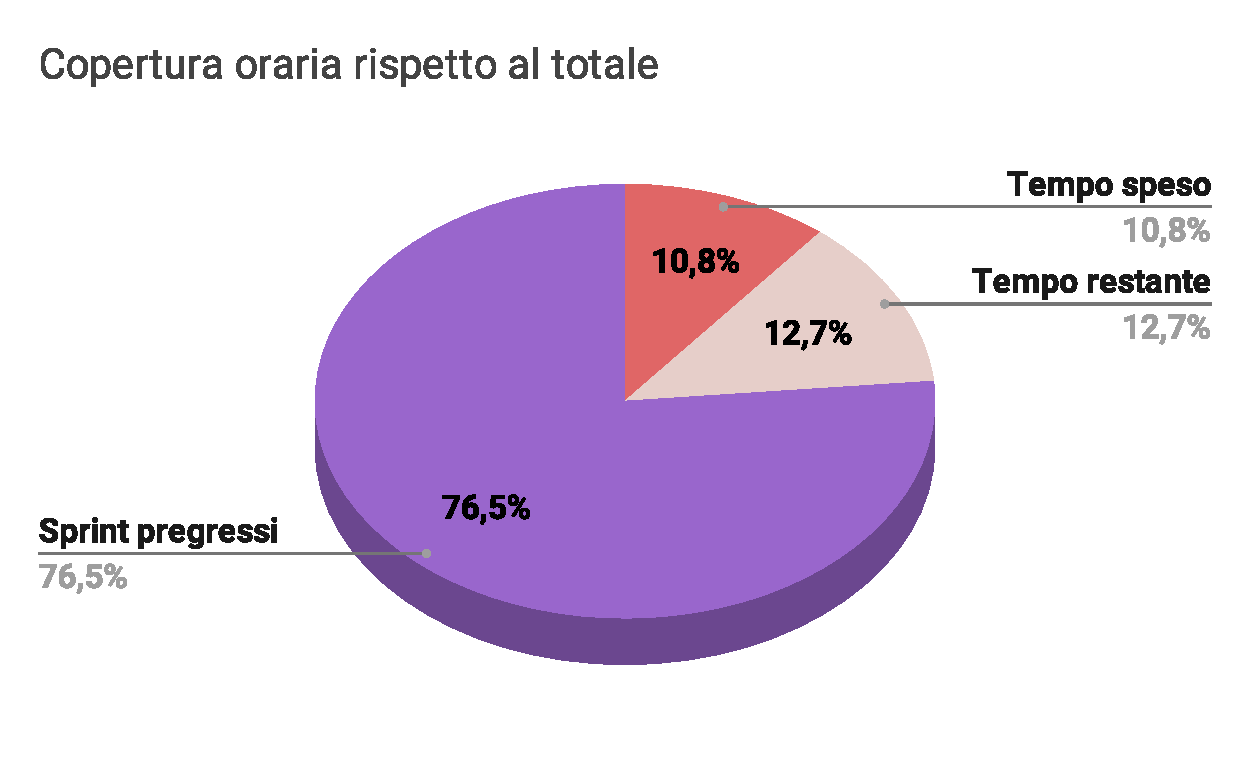
\includegraphics[width=0.90\textwidth]{assets/Consuntivo/Sprint-12/copertura_oraria.pdf}
    \caption{Sprint 12 - Areogramma del tempo speso (in ore) rispetto al totale}
  \end{figure}

  \begin{figure}[H]
    \centering
    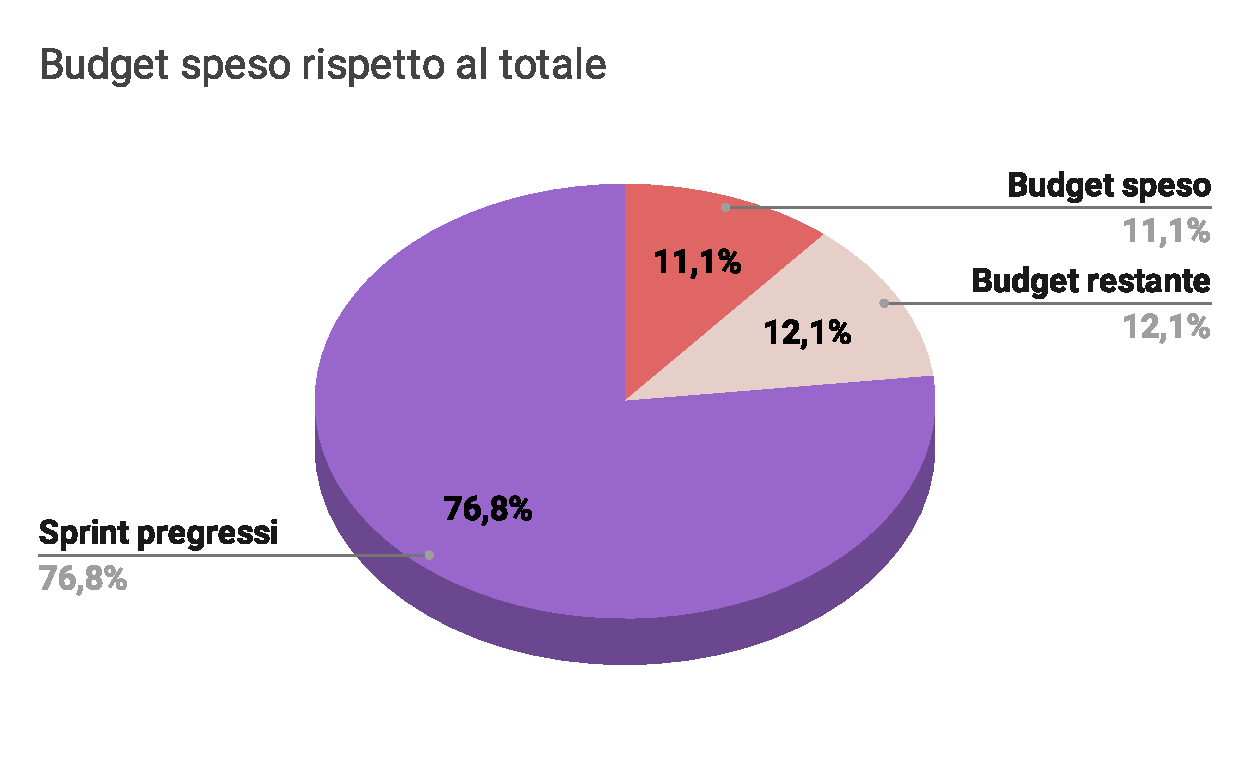
\includegraphics[width=0.90\textwidth]{assets/Consuntivo/Sprint-12/budget_speso.pdf}
    \caption{Sprint 12 - Areogramma del budget speso rispetto al totale}
  \end{figure}

  \begin{minipage}{\textwidth}
    Di seguito sono riportate le ore rimanenti per la coppia risorsa-ruolo:
    \begin{table}[H]
      \begin{tabularx}{\textwidth}{|c|*{6}{>{\centering}X|}c|}
        \hline
        \multicolumn{8}{|c|}{\textbf{Ore rimanenti per la coppia risorsa-ruolo}} \\
        \hline
        \textbf{Membro del team} & \textbf{Re} & \textbf{Am} & \textbf{An} & \textbf{Pt} & \textbf{Pr} & \textbf{Ve} & \textbf{Totale per persona} \\
        \hline
        Riccardo Cavalli & 0 & 1 & 1 & 2 & 4 & 3 & 11 \\
        \hline
        Raul Pianon & 1 & 1 & 1 & 0 & 5 & 2 & 10 \\
        \hline
        Martina Dall'Amico & 1 & 0 & 1 & 2 & 4 & 4 & 12 \\
        \hline
        Marco Cristo & 0 & 1 & 0 & 4 & 3 & 4 & 12 \\
        \hline
        Sebastiano Lewental & 2 & 0 & 1 & 2 & 4 & 3 & 12 \\
        \hline
        Mattia Zecchinato & 0 & 2 & 0 & 4 & 3 & 3 & 12 \\
        \hline
        Tommaso Stocco & 1 & 0 & 1 & 5 & 3 & 3 & 13 \\
        \hline
        \textbf{Totale ore per ruolo} & 5 & 5 & 5 & 19 & 26 & 22 & \textbf{82} \\
        \hline
      \end{tabularx}
      \caption{Sprint 12 - Ore rimanenti per la coppia risorsa-ruolo}
    \end{table}
  \end{minipage}

\subsubsection{Revisione delle attività}

Nell'arco del dodicesimo \glossario{sprint}, il team ha svolto le seguenti attività:
\begin{itemize}
  \item Completati test dei componenti \glossario{front-end};
  \item Completati test di unità e di integrazione \glossario{back-end};
  \item Avanzamento codifica back-end e front-end;
  \item Implementazione test di sistema;
  \item Registrazione dei test e del relativo esito nel \PdQ;
  \item Revisione del codice sorgente;
  \item Miglioramento algoritmo di ricerca semantica con \glossario{txtai};
  \item Completata sezione \glossario{debug} nel \MU;
  \item Stesura verbali interni;
  \item Stesura consuntivo \glossario{sprint} 11;
  \item Aggiornamento del documento di \ST\ nelle seguenti sezioni:
  \begin{itemize}
    \item Diagrammi delle classi;
    \item \glossario{DTO} (Data Transfer Objects);
    \item Adapter e porte;
    \item Core dell'applicazione;
    \item Design pattern utilizzati.
  \end{itemize}
  \item Aggiornamento e tracciamento dei requisiti;
  \item Aggiunti commenti alle suite di test;
  \item Miglioramento del controllo degli errori;
  \item Implementazione della funzionalità di ricerca dei \glossario{dizionari dati};
  \item Aggiunti test di sistema al workflow;
  \item Pubblicazione dell'immagine \glossario{Docker} del front-end su \glossario{GHCR};
  \item Risoluzione degli errori più comuni individuati da SonarCloud;
  \item Inserimento del badge di code coverage all'interno del \glossario{repository} ChatSQL;
  \item Aggiornamento del cruscotto di valutazione della qualità nel \PdQ.
\end{itemize}

\subsubsection{Retrospettiva}

\par Di seguito sono riportati i risultati del questionario di valutazione dello \glossario{sprint}:
\begin{itemize}
  \item Organizzazione dello sprint - Valutazione: 9;
  \item Conduzione dei meeting interni - Valutazione: 9;
  \item Impegno e partecipazione dei singoli membri - Valutazione: 9;
  \item Tutti i membri del team erano a conoscenza delle proprie mansioni;
  \item La numerosità delle riunioni è risultata adeguata per tutti i membri del gruppo;
  \item Le riunioni sono state organizzate con il giusto preavviso;
  \item Il rapporto medio tra ore spese e ore produttive è stato di 1.5.
\end{itemize}

\vspace{0.5\baselineskip}
\par A seguire le \textbf{analisi a posteriori} del dodicesimo \glossario{sprint}:
\begin{itemize}
  \item Durante lo sprint, il gruppo ha ampliato il documento di \ST, raggiungendo una struttura e un livello di dettaglio soddisfacenti. Inoltre, il team ha corretto alcuni errori relativi ai tipi di ritorno, ai parametri e alle relazioni tra le classi. Nel prossimo sprint, verranno integrate considerazioni approfondite sulle scelte progettuali, sia per il \glossario{front-end} che per il \glossario{back-end};
  \item Il team ha completato il tracciamento dei requisiti e la registrazione dei test. Di conseguenza, lo sprint successivo sarà dedicato al calcolo delle metriche e alla documentazione di quelle già calcolate;
  \item Il gruppo ha ultimato i test di unità e di integrazione sia per il front-end che per il back-end, ottenendo una copertura del codice superiore al 90\%. Inoltre, sono stati implementati tutti i test di sistema previsti dal \PdQ. Lo sviluppo dei test in parallelo alle attività di codifica ha permesso al team di conseguire gli obiettivi stabiliti con un anticipo rispetto alle previsioni iniziali;
  \item Uno dei problemi emersi negli sprint precedenti riguardava la scarsa documentazione del codice back-end. Per questo motivo, l'aggiunta dei commenti è stata definita come prioritaria per lo sprint 12. Una volta raggiunto un livello adeguato di completezza descrittiva, il team si è dedicato allo sviluppo delle funzionalità rimanenti;
  \item Il gruppo ha completato la redazione delle istruzioni per l'utilizzo dell'applicazione nel \MU. Sono state inoltre aggiunte delle immagini per migliorare la leggibilità e la comprensibilità del documento;
  \item Nonostante l'avvicinarsi dell'ultima sessione di esami, il team ha mantenuto un ritmo di lavoro adeguato, anche se non sempre costante. Il rapporto tra le ore impiegate e quelle realmente produttive è migliorato in modo significativo, evidenziando il crescente livello di efficienza conseguito nel corso del progetto;
  \item La configurazione del workflow su \glossario{GitHub} è stata completata. Questo ha permesso al gruppo di eseguire i test automatici in un unico flusso di lavoro, generando report e badge di stato.
\end{itemize}

\subsubsection{Aggiornamento pianificazione e preventivo}
\par Il team ha definito un piano d'azione per migliorare l'organizzazione e la produttività del prossimo \glossario{sprint}:
\begin{itemize}
  \item Programmazione di incontri informali per collaborare alla redazione della documentazione;
  \item Organizzazione di un incontro in presenza per esaminare lo stato di avanzamento in preparazione alla revisione \glossario{PB}.
\end{itemize}

\paragraph*{Pianificazione futura:}
\par Poiché i test di sistema sono stati implementati e integrati nel workflow, il team ha deciso di avviare la fase di collaudo. Pertanto, sarà organizzata una riunione con la \glossario{Proponente} per fornire un aggiornamento sullo stato del progetto.

\paragraph*{Preventivo "a finire" (\sezione{sec:stima_temporale}):}
\par Alla luce delle attività svolte, il gruppo intende rispettare il costo stimato per la realizzazione del progetto (con possibilità di risparmiare sul budget) e la data di consegna prevista per metà settembre.

\paragraph*{Gestione dei rischi (\sezione{sec:analisi_rischi}):}
\par Durante il dodicesimo \glossario{sprint}, i seguenti rischi sono stati gestiti con successo:
\begin{itemize}
  \item \textbf{RO6: Risorse disponibili ma non impiegate}: il team ha sovrastimato le risorse necessarie per le attività di progettazione, portando alcuni membri a disperdere ore potenzialmente produttive. Tuttavia, grazie alle competenze acquisite e alla collaborazione interna, il gruppo è riuscito a evitare ritardi nelle fasi di codifica e testing.
\end{itemize}